\documentclass[11pt]{beamer}

%%%% Parámetros

\usepackage{listings} % Include the listings-package
\usepackage[T1]{fontenc}
\usepackage[utf8]{inputenc}
\usepackage[english]{babel}
\usepackage{amsmath}
\usepackage{amssymb, amsfonts, latexsym, cancel}
\usepackage{float}
\usepackage{graphicx}
\usepackage{epstopdf}
\usepackage{subfigure}
\usepackage{hyperref}
%\usepackage{authblk}
\usepackage{blindtext}
\usepackage{booktabs} % Allows the use of \toprule, 
\usepackage{filecontents}
\usepackage{courier} %% Sets font for listing as Courier.
\usepackage{listings}

%%%%%%Parámetros

\lstset{
tabsize = 2, %% set tab space width
showstringspaces = false, %% prevent space marking in strings, string is defined as the text that is generally printed directly to the console
numbers = left, %% display line numbers on the left
commentstyle = \color{green}, %% set comment color
keywordstyle = \color{blue}, %% set keyword color
stringstyle = \color{red}, %% set string color
rulecolor = \color{black}, %% set frame color to avoid being affected by text color
basicstyle = \small \ttfamily , %% set listing font and size
breaklines = true, %% enable line breaking
numberstyle = \tiny,
}

%%%%%% Autor: Richart Escobedo Quispe

\usepackage{caption}
\DeclareCaptionFont{white}{\color{white}}
\DeclareCaptionFormat{listing}{\colorbox{gray}{\parbox{\textwidth}{#1#2#3}}}
\captionsetup[lstlisting]{format=listing,labelfont=white,textfont=white}
\definecolor{urlColor}{rgb}{0.06, 0.3, 0.57}
\definecolor{linkColor}{rgb}{0.57, 0.0, 0.04}
\definecolor{fileColor}{rgb}{0.0, 0.26, 0.26}
\hypersetup{
    colorlinks=true,
    linkcolor=linkColor,
    filecolor=fileColor,      
    urlcolor=urlColor,
}

%%%%% Autor : Richart Escobedo Quispe

\urlstyle{same}
\setbeamercovered{transparent}
%\usetheme{Boadilla}
\usetheme{CambridgeUS}
%\usetheme{Berkeley}
%\usetheme{Warsaw}
%\usetheme{Madrid}

%% Separación de Diapositivas

%%%% N°1

\title[JUnit]{\bf\Huge JUnit}
\subtitle{Fundamentals to programming I}

\author[agallegosco and fdelgadov]
{
Delgado Valencia Franco Andre \inst{1}
\\Gallegos Condori Anette Isabel \inst{2}
}
\institute[UNSA]
{
\inst{1}% 
System Engineering School\\
System Engineering and Informatic Department\\
Production and Services Faculty\\
San Agustin National University of Arequipa
}
\date[28/07/2020]{\scriptsize{28/07/2020}}

\titlegraphic{
\includegraphics[width=2.0cm]{img/logo_unsa.jpg}}

%\setbeamercovered{transparent} 
%\setbeamertemplate{navigation symbols}{} 
%\logo{:0}  
%\subject{}


\begin{document}

\begin{frame}
\titlepage
\end{frame}

%\begin{frame}
%\tableofcontents
%\end{frame}

%%%%N°2

\begin{frame}

\begin{center}

\includegraphics[width=10.0cm]{img/JUnit_logo.jpg}
\end{center}

\end{frame}

%%%%N°3

\begin{frame}{\textbf{Content}}

1. What is JUnit?
\\2. Implementation
\\3. Test-Driven Development
\\4. Examples

\begin{scriptsize}
\begin{itemize}
\item BlackJack
\item BlackJackTest
\item MissingChar
\item MissingCharTest
\item TablasDeVerdad
\item TablasDeVerdadTest
\item ADN
\item ADNTest
\end{itemize}
\end{scriptsize}

5. References

\end{frame}

%%%% N°4

\begin{frame}{\textbf{What is JUnit?}}

Tool specially designed to implement and automate the unit test relationship in \textbf{JAVA}.

\end{frame}

%%%% N°5

\begin{frame}{\textbf{Implementation}}

1. In a separate class
\begin{itemize}
\item The class inherits from \emph{org.junit.jupiter.api.Test}.
\item Each test case is implemented in a separate method.
\item Test case names begin with \emph{Test}.
\end{itemize}

\begin{center}
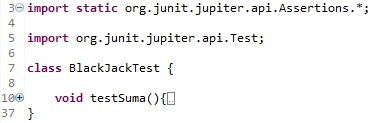
\includegraphics[width=9.0cm]{img/TestCase.jpg}
\end{center}

\end{frame}

%%%% N°6

\begin{frame}{\textbf{Implementation}}
2. Each test case invokes a series of methods in our class and checks the results obtained after invoking them.

\begin{itemize}
\item We create the test with \emph{@Test}.
\item Depending on the type and amount of data that were used in the class, they will be used in the Test.
\item \emph{AssertEquals()} methods checks that the two objects are equals or not.
\end{itemize}

\begin{center}
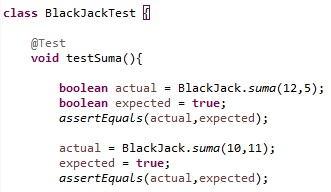
\includegraphics[width=5.0cm]{img/Test2.jpg} \quad 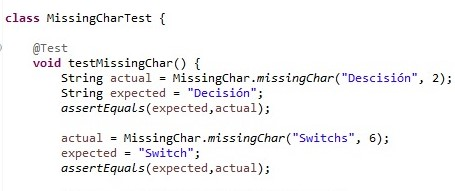
\includegraphics[width=5.5cm]{img/Test1.jpeg}
\end{center}

\begin{center}
{\small \textit{Note: The Test may vary depending on the class.}}
\end{center}

\end{frame}

%%%% N°7

\begin{frame}{\textbf{Implementation}}

3. Finally, we run the test cases in JUnit.

\begin{itemize}
\item If all cases work correctly:
\end{itemize}

\begin{center}
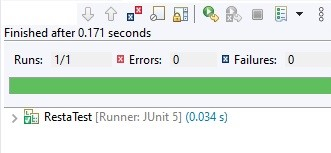
\includegraphics[width=8.0cm]{img/True.jpg}
\end{center}

\end{frame}

%%%% N°8

\begin{frame}{\textbf{Implementation}}

\begin{itemize}
\item If any test case fails:
\end{itemize}

\begin{center}
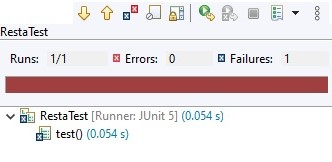
\includegraphics[width=8.0cm]{img/False.jpg}
\end{center}

\end{frame}

%%%% N°9

\begin{frame}{\textbf{Test-Driven Development}}
It consists of implementing unit test before even starting to write the code of a module.
\end{frame}

%%%% N°10

\begin{frame}{\textbf{Traditionally}}
\framesubtitle{\textit{Tests are carried out after.}}
Test cases are generally written after implementing the module whose operation they are intended to verify.
\end{frame}

%%%% N°11

\begin{frame}{\textbf{TDD}}
\framesubtitle{\textit{Test are prepared before you start writing the code.}}
First we write a test case. Then we write the necessary code for the test case to pass successfully.
\end{frame}

%%%% N°12

\begin{frame}{\textbf{Vantages}}

\begin{itemize}
\item If we write the test cases first, we define the requirements that we expect our application to meet.
\item When we write a test case. We think about the correct way to use a module that does not exist.
\item Test cases execution is done automatically.
\item Test cases allow us to lose the fear of making modifications to the code.
\item Test cases determine when our work done.
\end{itemize}
\end{frame}

%%%% N°13

\begin{frame}{\textbf{Software construction process}}
\framesubtitle{It's a cycle}
1. Add a new test case. \\
2. Run test cases.\\
3. Make small changes to the implementation.\\
4. Run test cases.\\
5. Improve code design.\\
6. Run test cases.\\
7. Return to the initial step.
\end{frame}

%%%% N°14

\begin{frame}

\begin{center}
\textbf{\bf\Huge Examples} 
\end{center}

\end{frame}

%%%% N°15

\begin{frame}{\textbf{BlackJack}}

\begin{center}
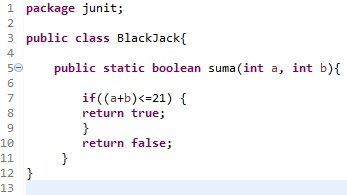
\includegraphics[width=7.0cm]{img/Ejemplo1.jpg}
\end{center}

\end{frame}

%%%% N°16

\begin{frame}{\textbf{BlackJackTest}}

\begin{center}
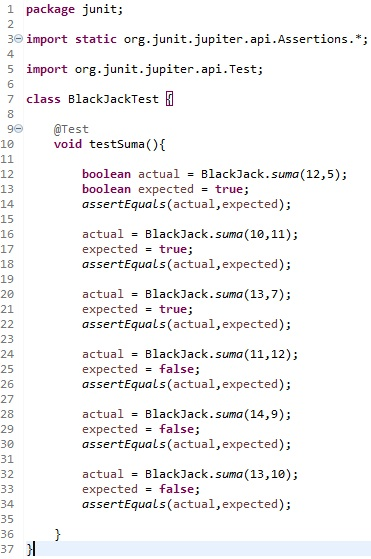
\includegraphics[width=4.5cm]{img/Prueba1.jpg}
\end{center}

\end{frame}

%%%% N°17

\begin{frame}{\textbf{MissingChar}}

\begin{center}
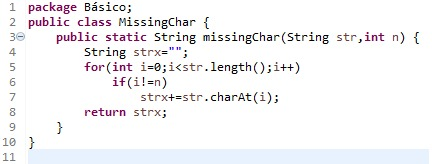
\includegraphics[width=8.0cm]{img/Ejemplo2.jpeg}
\end{center}

\end{frame}

%%%% N°18

\begin{frame}{\textbf{MissingCharTest}}

\begin{center}
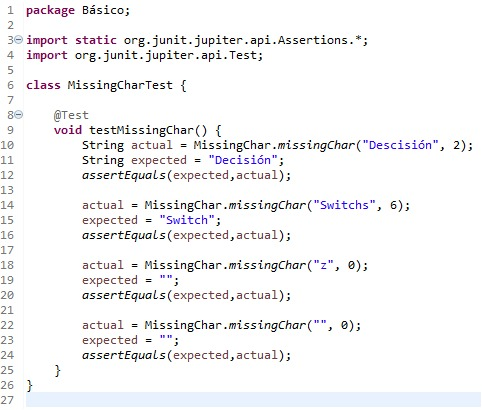
\includegraphics[width=7.0cm]{img/Prueba2.jpeg}
\end{center}

\end{frame}

%%%% N°19

\begin{frame}{\textbf{TablasDeVerdad}}

\begin{center}
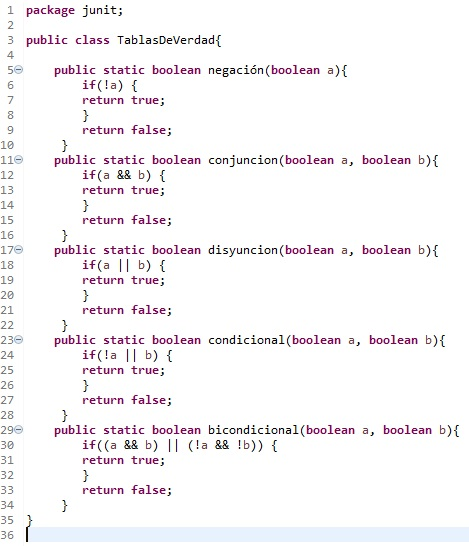
\includegraphics[width=6.4cm]{img/Ejemplo3.jpg}
\end{center}

\end{frame}

%%%% N°20

\begin{frame}{\textbf{TablasDeVerdadTest}}

\begin{center}
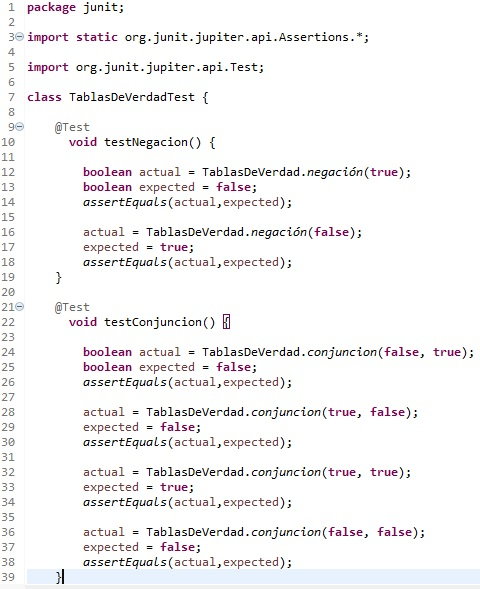
\includegraphics[width=6.0cm]{img/Prueba3.1.jpg}
\end{center}

\end{frame}

%%%% N°21

\begin{frame}{\textbf{TablasDeVerdadTest}}

\begin{center}
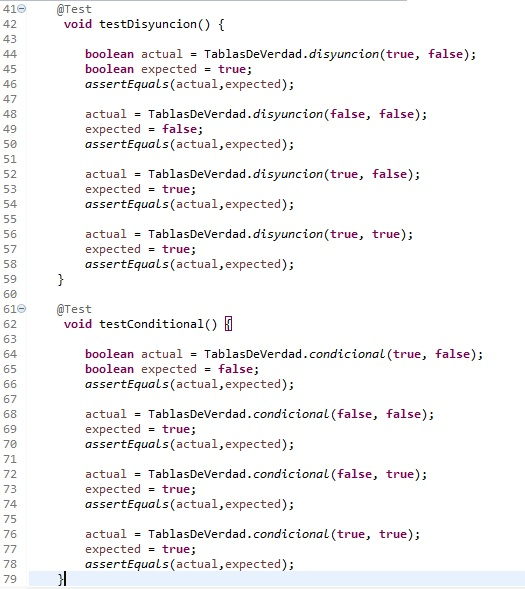
\includegraphics[width=6.0cm]{img/Prueba3.2.jpg}
\end{center}

\end{frame}

%%%% N°22

\begin{frame}{\textbf{TablasDeVerdadTest}}

\begin{center}
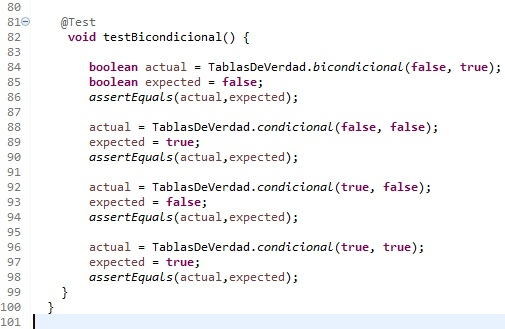
\includegraphics[width=8.0cm]{img/Prueba3.3.jpg}
\end{center}

\end{frame}

%%%% N°23

\begin{frame}{\textbf{ADN}}

\begin{center}
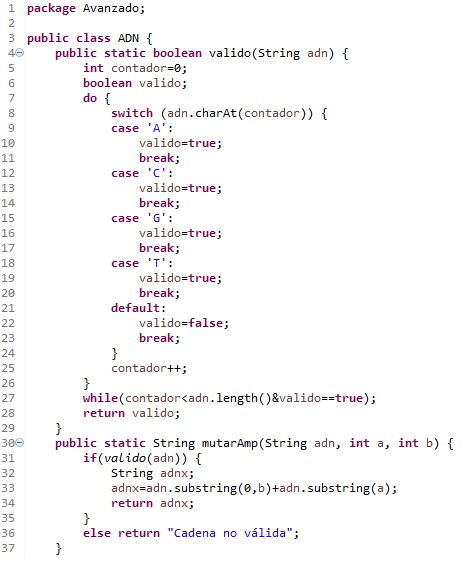
\includegraphics[width=6.0cm]{img/Ejemplo4.1.jpeg}
\end{center}

\end{frame}

%%%% N°24

\begin{frame}{\textbf{ADN}}

\begin{center}
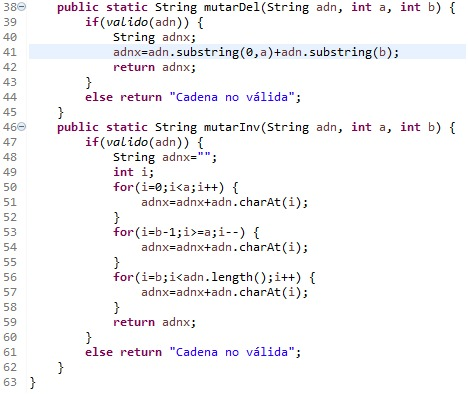
\includegraphics[width=5.0cm]{img/Ejemplo4.2.jpeg}
\end{center}

\end{frame}

%%%% N°25

\begin{frame}{\textbf{ADNTest}}

\begin{center}
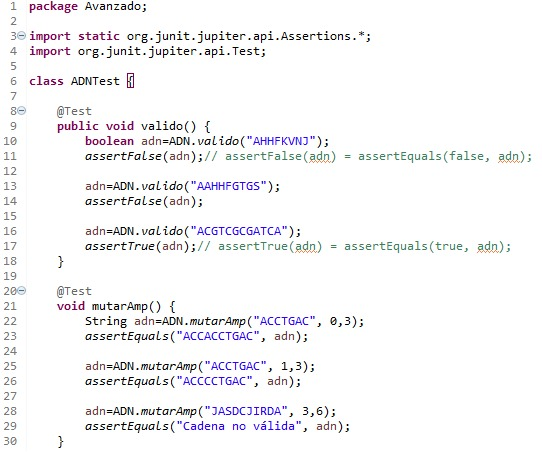
\includegraphics[width=8.0cm]{img/Prueba4.1.jpeg}
\end{center}

\end{frame}

%%%% N°26

\begin{frame}{\textbf{ADNTest}}

\begin{center}
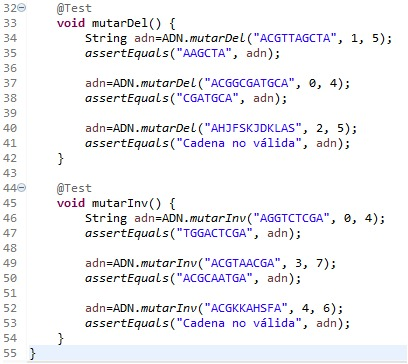
\includegraphics[width=7.5cm]{img/Prueba4.2.jpeg}
\end{center}

\end{frame}

%%%% N°27

\begin{frame}{\textbf{References}}

\begin{itemize}
\item[1] https://elvex.ugr.es/decsai/java/pdf/8C-JUnit.pdf
\item[2] https://junit.org/junit5/docs/current/user-guide/ \textit{[recommended visit]}
\end{itemize}

\end{frame}

%%%% N°28

\begin{frame}

\begin{center}
\textbf{\Huge Thanks for your attention}
\end{center}

\end{frame}

\end{document}
